\section{Аналитический обзор}


\subsection{Преобразование Фурье}{

Пусть $f : \mathbb{R} \to \mathbb{R}$ — непрерывно дифференцируемая функция. На основании теоремы о представлении функции в точке своим рядом Фурье можем, для любого $x \in \mathbb{R}$, записать её в виде ряда Фурье в промежутке $[-l, l]$: [6]

\[
f(x) = \frac{a_0}{2} + \sum_{n=1}^{\infty} \left( a_n \cos \frac{n \pi x}{l} + b_n \sin \frac{n \pi x}{l} \right), \tag{1.1}
\]

где
\[
a_n = \frac{1}{l} \int_{-l}^{l} f(t) \cos \frac{n \pi t}{l} \, dt, \quad n = 0, 1, 2, \dots, \tag{1.2}
\]
\[\begin{align}
b_n = \frac{1}{l} \int_{-l}^{l} f(t) \sin \frac{n \pi t}{l} \, dt, \quad n = 1, 2, \dots,   \tag{1.3}
\]

Разложение (1.1) обладает досадной несимметрией: его левая и правая части определены на всей числовой прямой, но разложение имеет место только в промежутке $[-l, l]$. Устраним этот недостаток, перейдя к пределу при $l \to \infty$. При этом ограничимся наглядными соображениями, оставив строгие рассуждения на потом.

Преобразуя (1.1), подставив вместо $a_n$ и $b_n$ их выражения (1.2):
\[
f(x) = \frac{1}{l} \int_{-l}^{l} f(t) \left[ \frac{1}{2} + \sum_{n=1}^{\infty} \left( \cos \frac{n \pi t}{l} \cos \frac{n \pi x}{l} + \sin \frac{n \pi t}{l} \sin \frac{n \pi x}{l} \right) \right] dt =
\]
\[
= \frac{1}{l} \int_{-l}^{l} f(t) \left[ 1 + \sum_{n=1}^{\infty} \cos \frac{n \pi (x - t)}{l} \right] dt = \frac{1}{l} \int_{-l}^{l} f(t) \sum_{n=-\infty}^{\infty} \cos \frac{n \pi (x - t)}{l} dt =
\]
\[
= \frac{1}{l} \int_{-l}^{l} f(t) \sum_{n=-\infty}^{\infty} \cos \left( \frac{n \pi}{l} (x - t) \right) dt. \tag{1.4}
\]

Тогда интеграл, входящий в первое слагаемое в , стремится к конечному пределу при $l \to \infty$, а само первое слагаемое стремится к нулю. Поскольку $\Delta_n = \frac{n \pi}{l} \to 0$ при $l \to \infty$, то выражение

\[
\sum_{n=-\infty}^{\infty} \cos \Delta_n (x - t) \tag{1.5}
\]
можно интерпретировать как сумму Римана интеграла[10]
\[
\int_{-\infty}^{+\infty} \cos y(x - t) \, dy.\tag{1.6}
\]
(Надо только иметь в виду, что это очень не строгое соображение; некоторого хода бы потому, что написанный интеграл заведомо расходится.)

В результате мы можем надеяться, что, переходя к пределу $l \to +\infty$ в выражении , мы получим
\[
f(x) = \frac{1}{\pi} \int_{-\infty}^{+\infty} f(t) \cos y(x - t) \, dy. \tag{1.7}   
\]
Меняя порядок интегрирования и раскладывая косинус по известной тригонометрической формуле, получаем
\[
f(x) = \frac{1}{\pi} \int_{-\infty}^{+\infty} \left[ f(t) \cos y t \, dt \cdot \cos y x + f(t) \sin y t \, dt \cdot \sin y x \right] dy,    \tag{1.8}
\]
или
\[
f(x) = \frac{1}{\pi} \int_{0}^{+\infty} \left[ \int_{-\infty}^{+\infty} f(t) \cos y t \, dt \cdot \cos y x + \int_{-\infty}^{+\infty} f(t) \sin y t \, dt \cdot \sin y x \right] dy, \tag{1.9}
\]
где
\[
a(y) = \int_{-\infty}^{+\infty} f(t) \cos y t \, dt, \tag{1.10}
\]
\[
b(y) = \int_{-\infty}^{+\infty} f(t) \sin y t \, dt. \tag{1.11}
\]

Отметим, что при наших предположениях оба интеграла в  и  сходятся, а интеграл в , в свою очередь, не является интегралом, расходящимся на бесконечности. В то же время мы можем надеяться, что формула (1.9) будет справедлива на всей прямой и будет играть роль разложения функции в ряд Фурье.



Правая часть формулы называется \textit{интегралом Фурье}, а сама формула  — \textit{интегральной формулой Фурье}. Функция $a : \mathbb{R} \to \mathbb{R}$, определённая формулой (1.10), называется \textit{косинус-преобразованием Фурье функции} $f$. Функция $b : \mathbb{R} \to \mathbb{R}$, определённая формулой (1.11), называется \textit{синус-преобразованием Фурье функции} $f$.

Обратите внимание, что формулы  напоминают уже привычные вам формулы разложения $2\pi$-периодической функции в ряд Фурье:

\[
f(x) = \frac{a_0}{2} + \sum_{n=1}^{\infty} \left( a_n \cos n x + b_n \sin n x \right), \tag{1.12}
\]
где
\[
a_n = \frac{1}{\pi} \int_{-\pi}^{\pi} f(t) \cos n t \, dt, \quad n = 0, 1, 2, \dots, \tag{1.13}
\]
\[
b_n = \frac{1}{\pi} \int_{-\pi}^{\pi} f(t) \sin n t \, dt, \quad n = 1, 2, \dots.   \tag{1.14}
\]
}
\textbf{Комплексная форма преобразования Фурье}{
    
Допустим, что функция $f : \mathbb{R} \to \mathbb{R}$ представима своим интегралом Фурье:

\[
f(x) = \int_0^{+\infty} \left[ a(y) \cos xy + b(y) \sin xy \right] \, dy. \tag{1.15}
\]

Подставим в (1.15) выражения для синуса и косинуса по формулам Эйлера:[10]

\[
\cos \varphi = \frac{e^{i \varphi} + e^{-i \varphi}}{2}, \quad \sin \varphi = \frac{e^{i \varphi} - e^{-i \varphi}}{2i}. \tag{1.16}
\]

В результате получим:

\[
f(x) = \int_0^{+\infty} \left[ a(y) \frac{e^{i xy} + e^{-i xy}}{2} + b(y) \frac{e^{i xy} - e^{-i xy}}{2i} \right] \, dy =
\]
\[
= \int_0^{+\infty} \left[ \frac{a(y) - i b(y)}{2} e^{i xy} + \frac{a(y) + i b(y)}{2} e^{-i xy} \right] \, dy. \tag{1.17}
\]

Непосредственно из определения функции $a(y)$ вытекает, что она является чётной:

\[
a(-y) = \frac{1}{\pi} \int_{-\infty}^{+\infty} f(t) \cos (-t y) \, dt = \frac{1}{\pi} \int_{-\infty}^{+\infty} f(t) \cos t y \, dt = a(y). \tag{1.18}
\]

Аналогично, функция $b(y)$ является нечётной. Учитывая эти обстоятельства, сделаем замену переменной $y \to -y$ в последнем интеграле в (1.19):

\[
f(x) = \int_0^{+\infty} \frac{a(y) - i b(y)}{2} e^{i xy} \, dy + \int_{-\infty}^0 \frac{a(-y) - i b(-y)}{2} e^{-i xy} \, dy =
\]
\[
= \int_{-\infty}^{+\infty} \frac{a(y) - i b(y)}{2} e^{i xy} \, dy. \tag{1.20}
\]

Используя формулу Эйлера $e^{i \varphi} = \cos \varphi + i \sin \varphi$  \tag{1.21} и определения  косинус- и синус-преобразования, можем записать:

\[
\frac{a(y) - i b(y)}{2} = \frac{1}{2\pi} \int_{-\infty}^{+\infty} f(t) e^{-i t y} \, dt. \tag{1.22}
\]

Таким образом, мы получили новую формулу, эквивалентную формуле (1.22):

\[
f(x) = \frac{1}{2\pi} \int_{-\infty}^{+\infty} \left[ \int_{-\infty}^{+\infty} f(t) e^{-i t y} \, dt \right] e^{i x y} \, dy. \tag{1.23}
\]

Правая часть последнего равенства называется \textit{комплексной формой интеграла Фурье}.
}

\textbf{Преобразование Фурье}{




\textbf{Лемма (Римана–Лебега для бесконечного промежутка).} Если \( a \in \mathbb{R} \) и \( f: (a, +\infty) \to \mathbb{R} \) абсолютно интегрируема на \((a, +\infty)\), [3] т.е. если

\[
\int_{a}^{+\infty} |f(x)| \, dx < +\infty, \tag{1.24}
\]

то

\[
\lim_{p \to +\infty} \int_{a}^{+\infty} f(x) \cos px \, dx = \lim_{p \to +\infty} \int_{a}^{+\infty} f(x) \sin px \, dx = 0. \tag{1.25}
\]

Мы примем это утверждение без доказательства, поскольку оно лишь техническими деталями отличается от леммы Римана–Лебега.




Функцию \( f: \mathbb{R} \to \mathbb{R} \) будем называть кусочно-гладкой, если она является кусочно-гладкой в смысле теории рядов Фурье на любом конечном промежутке \([a, b]\), т.е. если в \([a, b]\) найдётся конечное число точек \( a = x_0 < x_1 < \cdots < x_n = b \) таких, что в каждом открытом интервале \((x_j, x_{j+1})\) функция \( f \) непрерывно дифференцируема, а в каждой точке \( x_j \) у \( f \) существуют конечные пределы слева и справа
\[
f(x_j - 0) = \lim_{h \to 0^+} f(x_j - h), \quad f(x_j + 0) = \lim_{h \to 0^+} f(x_j + h), \tag{1.26}
\]
а также существуют и конечны следующие пределы, похожие на левую и правую производные
\[
\lim_{h \to 0^+} \frac{f(x_j - h) - f(x_j - 0)}{-h}, \quad \lim_{h \to 0^+} \frac{f(x_j + h) - f(x_j + 0)}{h}. \tag{1.27}
\]

\textbf{Теорема (о представимости функции в точке своим интегралом Фурье).} Пусть \( f: \mathbb{R} \to \mathbb{R} \) — кусочно-гладкая абсолютно интегрируемая функция. Тогда для любого \( x \in \mathbb{R} \) справедливо равенство
\[
\int_0^{+\infty} [a(y) \cos yx + b(y) \sin yx] \, dy = \frac{1}{2} [f(x + 0) + f(x - 0)], \tag{1.28}
\]
где
\[
a(y) = \frac{1}{\pi} \int_{-\infty}^{+\infty} f(t) \cos ty \, dt, \tag{1.29}
\]
\[
b(y) = \frac{1}{\pi} \int_{-\infty}^{+\infty} f(t) \sin ty \, dt. \tag{1.30}
\]

Другими словами, эта теорема означает, что интеграл Фурье кусочно-гладкой абсолютно интегрируемой функции равен полусумме её пределов слева и справа. В частности, в точке непрерывности функции он в точности равен значению функции.

\textbf{Доказательство.} Положим
\[
f_A(x) = \int_0^A [a(y) \cos yx + b(y) \sin yx] \, dy \tag{1.31}
\]
и убедимся, что \( f_A(x) \to [f(x + 0) + f(x - 0)]/2 \) при \( A \to +\infty \). \tag{1.32}



Для начала преобразуем \( f_A(x) \), подставив вместо \( a(y) \) и \( b(y) \) их выражения через интегралы и воспользовавшись тригонометрической формулой для косинуса разности:
\[
f_A(x) = \frac{1}{\pi} \int_0^A \left\{ \int_{-\infty}^{+\infty} f(t) [\cos ty \cdot \cos yx + \sin ty \cdot \sin yx] \, dt \right\} \, dy
\]
\[
= \frac{1}{\pi} \int_0^A \left\{ \int_{-\infty}^{+\infty} f(t) \cos y(t - x) \, dt \right\} \, dy. \tag{1.33}
\]
Изменив порядок интегрирования в последнем выражении, получим
\[
f_A(x) = \frac{1}{\pi} \int_{-\infty}^{+\infty} \left[ f(t) \int_0^A \cos y(t - x) \, dy \right] \, dt. \tag{1.34}
\]

Для обоснования законности изменения порядка интегрирования в данном случае естественно использовать теорему Фубини: если функция интегрируема по совокупности переменных, то все её повторные интегралы существуют и не только равны между собой, но равны и её кратному интегралу. В нашем случае обосновать законность изменения порядка интегрирования как раз и значит доказать равенство повторных интегралов. Таким образом, всё дело упирается в интегрируемость функции двух переменных \((t, y) \mapsto f(t) \cos y(t - x)\) по множеству \(\mathbb{R} \times [0, A]\). Поскольку всякая абсолютно интегрируемая функция интегрируема, то нам достаточно доказать, что модуль этой функции интегрируем. Однако модуль — величина неотрицательная, а из курса математического анализа известно, что если для неотрицательной функции нескольких переменных сходится хоть один повторный интеграл, то эта функция интегрируема по совокупности всех переменных. Следовательно, для наших целей достаточно установить сходимость следующего повторного интеграла
\[
\int_{-\infty}^{+\infty} \left[ \int_0^A |f(t) \cos y(t - x)| \, dy \right] \, dt, \tag{1.35}
\]
сходимость которого вытекает из следующих очевидных выкладок:
\[
\int_{-\infty}^{+\infty} \left[ \int_0^A |f(t) \cos y(t - x)| \, dy \right] \, dt \leq
\]
\[
\leq \int_{-\infty}^{+\infty} |f(t)| \left[ \int_0^A |\cos y(t - x)| \, dy \right] \, dt \leq A \int_{-\infty}^{+\infty} |f(t)| \, dt < +\infty, \tag{1.36}
\]


Последнее неравенство написано в силу условия теоремы, согласно которому \( f \) абсолютно интегрируема. Тем самым мы завершили обоснование законности изменения порядка интегрирования и доказали равенство (1.31).

Преобразуем формулу (1.36):

\[
f_A(x) = \frac{1}{\pi} \int_{-\infty}^{+\infty} \left[ f(t) \int_0^A \cos y(t-x) \, dy \right] dt
\]

\[
= \frac{1}{\pi} \int_{-\infty}^{+\infty} \left\{ f(t) \frac{\sin y(t-x)}{t-x} \bigg|_{y=0}^{y=A} \right\} dt
\]

\[
= \frac{1}{\pi} \int_{-\infty}^{+\infty} f(t) \frac{\sin A(t-x)}{t-x} \, dt = \frac{1}{\pi} \int_{-\infty}^{+\infty} f(x+u) \frac{\sin Au}{u} \, du. \tag{1.37}
\]

Последнее равенство здесь получено с помощью линейной замены переменной \( t-x = u \). Пользуясь аддитивностью, разобьём последний интеграл на два (по промежуткам \((-∞, 0)\) и \((0, +∞)\), соответственно) и сделаем в первом из них замену \( u \to -u \):

\[
F_A(x) = \frac{1}{\pi} \int_{-\infty}^{+\infty} f(x+u) \frac{\sin Au}{u} \, du
\]

\[
= \frac{1}{\pi} \int_{-\infty}^{0} f(x+u) \frac{\sin Au}{u} \, du + \frac{1}{\pi} \int_{0}^{+\infty} f(x+u) \frac{\sin Au}{u} \, du
\]

\[
= \frac{1}{\pi} \int_{0}^{+\infty} \frac{f(x+u) + f(x-u)}{u} \sin Au \, du
\]

\[
= \frac{1}{\pi} \int_{0}^{1} \frac{f(x+u) + f(x-u)}{u} \sin Au \, du + \frac{1}{\pi} \int_{1}^{+\infty} \frac{f(x+u) + f(x-u)}{u} \sin Au \, du. \tag{1.38}
\]

Обозначим первый из этих интегралов через \( I_1 \), а второй через \( I_2 \).



Поскольку
\[
\int_{1}^{+\infty} \left| \frac{f(x + u) + f(x - u)}{u} \right| \, du \tag{1.39}

\int_{1}^{+\infty} |f(x + u)| \, du + \int_{1}^{+\infty} |f(x - u)| \, du \tag{1.40}

2 \int_{-\infty}^{+\infty} |f(v)| \, dv < +\infty, \tag{1.41}
\]
то функция \( u \mapsto \frac{f(x + u) + f(x - u)}{u} \) абсолютно интегрируема по промежутку \( [1, +\infty) \), и к \( I_2 \) можно применить лемму Римана–Лебега для бесконечного промежутка. Следовательно, \( I_2 \to 0 \) при \( A \to +\infty \).

Подобное рассуждение неприменимо к интегралу \( I_1 \), поскольку пока мы не в состоянии гарантировать интегрируемость функции \( u \mapsto \frac{f(x + u) + f(x - u)}{u} \) в окрестности нуля. Исследуем \( I_1 \) более детально, для чего прибавим и вычтем предельные значения \( f(x + u) \) и \( f(x - u) \) в числителе подынтегрального выражения:
\[
\begin{align*}
I_1 = & \, \frac{1}{\pi} \int_0^1 \frac{f(x + u) + f(x - u)}{u} \sin(Au) \, du \\
= & \, \frac{1}{\pi} \int_0^1 \frac{f(x + u) - f(x + 0)}{u} \sin(Au) \, du \\
& + \frac{1}{\pi} \int_0^1 \frac{f(x - u) - f(x - 0)}{u} \sin(Au) \, du \\
& + \frac{1}{\pi} \int_0^1 \frac{f(x + 0) + f(x - 0)}{u} \sin(Au) \, du. \tag{1.42}
\end{align*}
\]

Поскольку \( f \) — кусочно гладкая функция [11], то интервал \( [0, 1] \) можно разбить на конечное число открытых промежутков \( (x_j, x_{j+1}) \), на каждом из которых функции \( \frac{f(x + u) + f(x + 0)}{u} \) и \( \frac{f(x - u) + f(x - 0)}{u} \) непрерывно дифференцируемы, а в каждой из концевых точек \( x_j \) имеют конечные пределы слева и справа. Особо подчеркнём, что они имеют конечные пределы в точке \( x_j = 0 \) справа, поскольку существование и конечность этих пределов специально оговаривается в определении кусочно-гладкой функции. Учитывая такую структуру функций \( \frac{f(x + u) + f(x + 0)}{u} \) и \( \frac{f(x - u) + f(x - 0)}{u} \), заключаем, что обе они абсолютно интегрируемы на интервале \( [0, 1] \). Следовательно, по лемме Римана–Лебега, первые два слагаемых в  стремятся к нулю при \( A \to +\infty \). 


преобразуем с помощью линейной замены переменной \( Au = v \):
\[
\frac{1}{\pi} \int_0^1 \frac{f(x+0) + f(x-0)}{u} \sin(Au) \, du = \frac{f(x+0) + f(x-0)}{\pi} \int_0^A \frac{\sin v}{v} \, dv. \tag{1.43}
\]
Из курса математического анализа вы знаете, что интеграл
\[
\int_0^{+\infty} \frac{\sin v}{v} \, dv, \tag{1.44}
\]
называемый интегралом Дирихле, сходится, и его значение равно \( \frac{\pi}{2} \). Таким образом, при \( A \to +\infty \) третье слагаемое в уравнении (11) стремится к числу \( \frac{f(x+0) + f(x-0)}{2} \).

Окончательно получаем
\[
\lim_{A \to +\infty} f_A(x) = \lim_{A \to +\infty} I_1 + \lim_{A \to +\infty} I_2 = \frac{f(x+0) + f(x-0)}{2}, \tag{1.45}
\]
что и завершает доказательство теоремы.

Отметим, что существуют и другие условия, гарантирующие для данной точки совпадение значения интеграла Фурье со значением представляемой им функции. Однако следует иметь в виду, что только непрерывности и абсолютной интегрируемости функции для этого недостаточно.



}

   
\textbf{Синус- и косинус- преобразования Фурье}
 {
  
Пусть функция \( f : \mathbb{R} \to \mathbb{R} \) представима своим интегралом Фурье.[11]  Тогда для всех \( x \in \mathbb{R} \) имеем
\[
f(x) = \int_0^{+\infty} [a(y) \cos(yx) + b(y) \sin(yx)] \, dy, \tag{1.47}
\]
где
\[
a(y) = \frac{1}{\pi} \int_{-\infty}^{+\infty} f(t) \cos(yt) \, dt, \tag{1.48}
\]
\[
b(y) = \frac{1}{\pi} \int_{-\infty}^{+\infty} f(t) \sin(yt) \, dt. \tag{1.49}
\]

Если, кроме того, функция \( f \) чётная, то подынтегральная функция в  оказывается чётной, а значит, этот интеграл можно заменить удвоенным интегралом по половинному промежутку. Подынтегральная функция в (1.49) при этом оказывается нечётной, и интеграл в (1.49) зануляется для всех \( y \). Поэтому для чётной функции вместо (1.47)–(1.49) мы получаем следующие более простые и симметричные формулы:
\[
f(x) = \int_0^{+\infty} a(y) \cos(yx) \, dy, \tag{1.50}
\]
\[
a(y) = \frac{2}{\pi} \int_0^{+\infty} f(t) \cos(yt) \, dt. \tag{1.51}
\]

Аналогично, формулы (1.49)–(1.51) упрощаются и в случае, когда функция \( f \) нечётная. При этом результат выглядит так:
\[
f(x) = \int_0^{+\infty} b(y) \sin(yx) \, dy,  \tag{1.52}
\]
\[
b(y) = \frac{2}{\pi} \int_0^{+\infty} f(t) \sin(yt) \, dt. \tag{1.43}
\]

Предположим далее, что функция \( f \) задана лишь на полупрямой \( (0, +\infty) \). Можно ли представить её интегралом Фурье? Конечно, можно. Нужно лишь предварительно продолжить её разумным образом на всю прямую. Возникающий при этом произвол в выборе продолжения можно использовать для упрощения формул. В самом деле, продолжив функцию \( f : (0, +\infty) \to \mathbb{R} \) чётным образом, мы, естественно, придём к формулам . При этом функция \( a \), построенная по формуле (4.6), называется прямым косинус-преобразованием Фурье функции \( f \), а функция \( f \), построенная по формуле (4.6), называется обратным косинус-преобразованием Фурье функции . Обратите внимание ещё раз на то, что прямое и обратное косинус-преобразования Фурье различаются лишь числовым множителем.

Аналогично, продолжив функцию \( f : (0, +\infty) \to \mathbb{R} \) нечётным образом, мы получим для её интеграла Фурье формулы .

 }
\textbf{Геометрический смысл преобразования Фурье}  {
    Обозначим функцию, генерирующую сигнал, как \( g(t_k) \).[7] Здесь \( t_k \) означает время снятия \( k \)-го отсчёта сигнала, так как величина сигнала меняется во времени. Отобразим \( g(t_k) \) на комплексную плоскость. Для этого введём радиус-вектор, который равномерно вращается по часовой стрелке. Его длина в каждый момент времени равна модулю значения сигнала, а частота вращения выбирается произвольным образом. Вращение радиус-вектора с частотой \( \vartheta \) описывается двумя функциями: одна отвечает за изменение горизонтальной координаты, а другая – за вертикальную.

\[
x(t_k) = \cos(2\pi \vartheta t_k) \tag{1.44}
\]
\[
y(t_k) = \sin(2\pi \vartheta t_k) \tag{1.45}
\]

Получающаяся точка с координатами \( (x, y) \) вращается против часовой стрелки вокруг начала координат на постоянном единичном расстоянии, делая \( \vartheta \) оборотов за одну секунду. Чтобы получить координаты точек контура намотки функции \( g(t) \) на плоскость, нужно умножить координаты вращающейся точки на значение функции \( g(t) \):

\[
X(t_k) = g(t_k) \cdot \cos(2\pi \vartheta t_k) \tag{1.46}
\]
\[
Y(t_k) = g(t_k) \cdot \sin(2\pi \vartheta t_k) \tag{1.47}
\]

А чтобы получить координаты центра массы для частоты намотки \( \vartheta \), нужно посчитать средние значения для иксов и игреков отдельно:

\[
M_x(\vartheta) = \frac{1}{N} \sum_{k=0}^{N-1} g(t_k) \cdot \cos(2\pi \vartheta t_k) \tag{1.48}
\[
M_y(\vartheta) = \frac{1}{N} \sum_{k=0}^{N-1} g(t_k) \cdot \sin(2\pi \vartheta t_k) \tag{1.49}
\]

Здесь \( N \) – количество значений входного сигнала. В реальности это – значения сигнала, выдаваемые АЦП. Чтобы перейти к координатам на комплексной плоскости, умножим выражение для вертикальной составляющей \( M_y \) на мнимую единицу \( i \), соответствующую вертикальной составляющей в представлении комплексного числа на плоскости. Получаем формулу для дискретного преобразования Фурье:

\[
M(\vartheta) = \frac{1}{N} \sum_{k=0}^{N-1} g(t_k) \cdot \left(\cos(2\pi \vartheta t_k) + i \cdot \sin(2\pi \vartheta t_k)\right) \tag{1.50}
\]

Выражение в скобках соответствует формуле Эйлера. Заменяем косинус и синус на формулу Эйлера:

\[
e^{ix} = \cos(x) + i \cdot \sin(x) \tag{1.51}

\]

Тогда:

\[
M(\vartheta) = \frac{1}{N} \sum_{k=0}^{N-1} g(t_k) \cdot e^{2\pi i \vartheta t_k} \ \tag{1.52}
\]

В пределе можно перейти к интегральному представлению:

\[
M(\vartheta) = \frac{1}{t_2 - t_1} \int_{t_1}^{t_2} g(t) \cdot e^{2\pi i \vartheta t} \, dt \tag{1.53}
\]

В литературе встречаются разные определения этого преобразования, отличающиеся множителем перед интегралом и знаком перед \( i \), влияющим на направление намотки сигнала. Минус меняет намотку в направлении часовой стрелки. Классическое представление преобразования Фурье на бесконечном интервале выглядит так:

\[
f(\omega) = \frac{1}{\sqrt{2\pi}} \int_{-\infty}^{+\infty} f(x) e^{-i\omega x} \, dx    \tag{1.54}
\]

Здесь видно, что поменялся нормировочный множитель перед интегралом, частота \( \vartheta \) заменена на циклическую частоту \( \omega \), и поставлен «минус» перед мнимой единицей \( i \).
}




\subsection{Дискретное преобразование Фурье}{
    Пусть исходный дискретный сигнал \( s_{\text{д}}(t) \) ограничен во времени и содержит \( N \) ненулевых отсчётов, взятых с интервалом дискретизации \( T \) секунд.[6] Данное предположение на практике всегда выполняется, потому что мы не можем получить бесконечное число отсчётов сигнала. Тогда длительность дискретного сигнала равна \( NT \) секунд, и \( s_{\text{д}}(t) \) можно записать как:[6]

\begin{equation}
s_{\text{д}}(t) = \sum_{n=0}^{N-1} s_n \delta(t - nT), \tag{2.1}
\end{equation}

где \( \delta(t) \) — дельта-функция Дирака.

Известно, что дискретным, или, как ещё говорят, линейчатым спектром, обладают периодические сигналы. При этом дискретный спектр получается путём разложения в ряд Фурье периодического сигнала. Значит, чтобы получить дискретный спектр, надо сделать исходный дискретный сигнал периодическим путём повторения данного сигнала во времени бесконечное количество раз с некоторым периодом \( P \), кратным интервалу дискретизации \( T \). Мы можем осуществить такое периодическое повторение сигнала, потому что его длительность конечна.

Графически процесс повторения сигнала во времени представлен на рисунке 1.
\begin{center}
    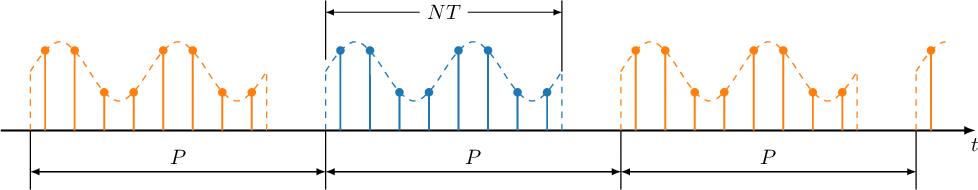
\includegraphics[width=1.0\textwidth]{dft_fig2.png}  
    \end{center}
    Повторять сигнал можно с различным периодом \( P \), однако необходимо, чтобы период повторения был больше или равен длительности сигнала \( P \geq NT \), чтобы сигнал и его периодические повторения не перекрывались во времени.

    При этом минимальный период повторения сигнала, при котором сигнал и его повторения не накладываются друг на друга, равен 
    
    \[
    P_{\text{min}} = NT \, \text{секунд}.
    \]
    
    Повторение сигнала с минимальным периодом \( P_{\text{min}} = NT \) показано на рисунке 2.]\

\begin{center}
    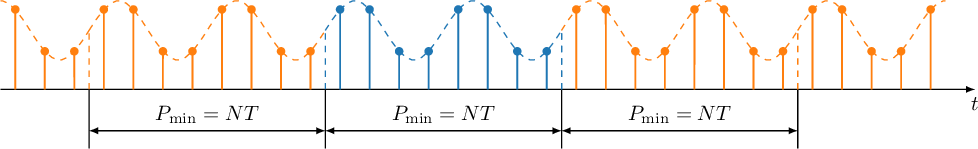
\includegraphics[width=1.0\textwidth]{dft_fig3.png}  
    \end{center}
}
При разложении периодически повторенного сигнала (1) в ряд Фурье получим дискретный спектр \( S(k \Delta \omega) \), состоящий из гармоник, кратных \( \Delta\omega = \frac{2\pi}{P_{\text{min}}} = \frac{2\pi}{NT} \) рад/с, где \( k \) — произвольное целое число. Тогда коэффициенты разложения в ряд Фурье \( S(k \Delta \omega) \) равны:

\begin{equation}
\label{eq2}
S(k \Delta \omega) = \frac{1}{P_{\text{min}}} \int_{P_{\text{min}}} s(t) e^{-jk\Delta\omega t} dt \tag{2.2}
\end{equation}

Подставим (2.1) в (2.2):

\begin{equation}
\label{eq3}
S(k \Delta \omega) = \frac{1}{P_{\text{min}}} \int_{P_{\text{min}}} \sum_{n=0}^{N-1} s(nT) \delta(t - nT) e^{-jk\Delta\omega t} dt \tag{2.3}
\end{equation}

Поменяем местами операции суммирования и интегрирования и применим фильтрующее свойство дельта-функции:

\begin{equation}
\label{eq4}
S(k \Delta \omega) = \frac{1}{P_{\text{min}}} \sum_{n=0}^{N-1} s(nT) e^{-jk\Delta\omega nT} \tag {2.4}
\end{equation}

Учтем, что \( \Delta \omega T = \frac{2\pi}{N} \), тогда окончательно можно записать:

\begin{equation}
\label{eq5}
S(k \Delta \omega) = \frac{1}{N} \sum_{n=0}^{N-1} s(nT) e^{-j\frac{2\pi}{N}kn} \tag{2.5}
\end{equation}

Заметим, что показатели комплексных экспонент в выражении \eqref{eq5} не зависят от интервала дискретизации \( T \), а только от индексов \( n \) и \( k \), указывающих порядковый номер временного и спектрального отсчета. Это очень полезное свойство, которое позволяет реализовать универсальную программу расчета для любой частоты дискретизации, используя лишь индексы \( n \) и \( k \).

Выражение \eqref{eq5} справедливо для любого целого \( k \), однако вспомним, что исходный сигнал \( s_{\text{д}}(t) \) был дискретным, поэтому спектр \( S(k \Delta \omega) \) является периодическим и повторяется каждые \( N \) отсчетов. Это очень легко проверить, если подставить в \eqref{eq5} вместо \( k \), например, \( k+N \), тогда:

\begin{equation}
\label{eq6}
S((k+N)\Delta \omega) = S(k \Delta \omega)
\end{equation}

Таким образом, нет необходимости рассчитывать спектральные отсчеты для всех индексов \( k \), а достаточно рассчитать лишь \( N \) спектральных отсчетов \( S(k \Delta \omega), k = 0 \ldots N-1 \).

Выражение \eqref{eq5} является дискретным преобразованием, которое ставит в соответствие \( N \) отсчетам исходного дискретного сигнала \( s(nT) \), \( N \) спектральных отсчетов \( S(k \Delta \omega) \) на одном периоде повторения спектра.

Заметим, что \eqref{eq5} является именно спектром, а не спектральной плотностью, потому что мы получили \( S(k \Delta \omega) \) как результат разложения в ряд Фурье. Это означает, что единицы измерения \( S(k \Delta \omega) \) совпадают с единицами измерения исходного сигнала.

Если мы будем оперировать только с индексами входного сигнала и спектральных отсчетов (положив \( T = 1 \)), то получим выражение дискретного преобразования Фурье:

\begin{equation}
\label{eq7}
S(k) = \frac{1}{N} \sum_{n=0}^{N-1} s(n) e^{-j\frac{2\pi}{N}kn} \tag{2.6}
\end{equation}

Выражение прямого ДПФ не содержит множителя \( \frac{1}{N} \), в отличие от \eqref{eq7}. Забегая вперед, скажем, что мы тоже перенесем этот множитель \( \frac{1}{N} \) в выражение обратного дискретного преобразования Фурье.

\textbf{Обратное дискретное преобразование Фурье}

При рассмотрении обратного дискретного преобразования Фурье (ОДПФ) [11] применим тот же прием, что мы использовали в предыдущем разделе при выводе формулы обратного дискретно-временного преобразования Фурье. Учтем, что ДПФ возвращает один период дискретного периодического спектра \( S(k \Delta \omega), k = 0 \ldots N-1 \). Тогда дискретный спектр ДПФ на одном периоде можно записать, используя дельта-функцию:

\begin{equation}
\label{eq8}
S_{\text{дпф}}(\omega) = \sum_{k=0}^{N-1} S(k \Delta \omega) \delta(\omega - k\Delta \omega) \tag{2.7}
\end{equation}

Спектр \( S_{\text{дпф}}(\omega) \) является \( \Omega \)-периодической функцией и может быть разложен в ряд Фурье вида:

\begin{equation}
\label{eq9}
S_{\text{дпф}}(\omega) = \sum_{m=-\infty}^{\infty} p(\xi_m) e^{j\omega \xi_m} \tag{2.8}
\end{equation}

где \( \xi_m = \frac{2\pi m}{\Omega} = mT \) имеет смысл временных отсчетов, так как мы раскладываем в ряд функцию частоты, а \( p(\xi_m) \) — коэффициенты разложения в ряд Фурье:

\begin{equation}
\label{eq10}
p(\xi_m) = \frac{1}{\Omega} \int_{-\Omega/2}^{\Omega/2} S_{\text{дпф}}(\omega) e^{-j\omega \xi_m} d\omega \tag{2.9}
\end{equation}

Подставим в \eqref{eq10} выражение \eqref{eq8}:

\begin{equation}
\label{eq11}
p(\xi_m) = \frac{1}{\Omega} \int_{-\Omega/2}^{\Omega/2} \sum_{k=0}^{N-1} S(k \Delta \omega) \delta(\omega - k\Delta \omega) e^{-j\omega \xi_m} d\omega \tag{2.10}
\end{equation}

Поменяем местами операторы интегрирования и суммирования и применим фильтрующее свойство дельта-функции:

\begin{equation}
\label{eq12}
p(\xi_m) = \frac{1}{\Omega} \sum_{k=0}^{N-1} S(k \Delta \omega) e^{-jk\Delta \omega \xi_m} \tag{2.11}
\end{equation}

Подставим в \eqref{eq12} выражение \eqref{eq5} для \( S(k \Delta \omega) \):

\begin{equation}
\label{eq13}
p(\xi_m) = \frac{1}{\Omega} \sum_{k=0}^{N-1} \frac{1}{N} \sum_{n=0}^{N-1} s(nT) e^{-j\frac{2\pi}{N}kn} e^{-j\frac{2\pi}{N}km} \tag{2.12}
\end{equation}

Поменяем порядок суммирования и объединим показатели экспонент:

\begin{equation}
\label{eq14}
p(\xi_m) = \frac{1}{N} \sum_{n=0}^{N-1} s(nT) \sum_{k=0}^{N-1} e^{-j\frac{2\pi}{N}k(n+m)} \tag{2.13}
\end{equation}

Можно заметить, что сумма комплексных экспонент равна

\begin{equation}
\label{eq15}
\sum_{k=0}^{N-1} e^{-j\frac{2\pi}{N}k(n+m)} =
\begin{cases} 
N, & n = -m \, (\text{mod } N) \\
0, & n \neq -m \, (\text{mod } N) \tag{2.14}
\end{cases}
\end{equation}

Тогда от суммы \eqref{eq14}, с учетом \eqref{eq15}, остается лишь одно слагаемое при \( n = -m \):

\begin{equation}
\label{eq18}
p(\xi_m) = s(-mT)
\end{equation}

Возвращаясь к выражению \eqref{eq12}, с учетом \eqref{eq18}, можно окончательно записать:

\begin{equation}
\label{eq19}
s(nT) = \sum_{k=0}^{N-1} S(k \Delta \omega) e^{j\frac{2\pi}{N}kn} \tag{2.15}
\end{equation}

Опустив \( \Delta \omega \) и приняв \( T = 1 \), можно перейти к паре дискретных преобразований Фурье, которые оперируют только с индексами входного дискретного сигнала \( s(n) \) и его спектра \( S(k) \):

\begin{equation}
\label{eq20}
S(k) = \sum_{n=0}^{N-1} s(n) e^{-j\frac{2\pi}{N}kn}, \quad \tag{2.16}
s(n) = \frac{1}{N} \sum_{k=0}^{N-1} S(k) e^{j\frac{2\pi}{N}kn} \tag{2.17}
\end{equation}

Заметим, что в \eqref{eq20} мы ограничили индексы \( n \) и \( k \) значением \( N-1 \). На самом деле этого можно не делать, но из-за периодического характера сигнала и спектра их значения будут повторяться с периодом \( N \).

Важно отметить, что на практике гораздо чаще требуется рассчитывать прямое ДПФ, чем обратное. Поэтому принято нормировочный множитель \( \frac{1}{N} \) учитывать в обратном преобразовании, а не в прямом. Тогда пару ДПФ можно переписать в виде:

\begin{equation}
\label{eq21}
S(k) = \sum_{n=0}^{N-1} s(n) e^{-j\frac{2\pi}{N}kn}, \quad \tag{2.18}
s(n) = \frac{1}{N} \sum_{k=0}^{N-1} S(k) e^{j\frac{2\pi}{N}kn} \tag{2.19}
\end{equation}

Именно в виде \eqref{eq21} принято записывать выражения прямого и обратного ДПФ.
}
\textbf {Быстрое преобразование Фурье}{
    Быстрое преобразование Фурье (БПФ) — это эффективный алгоритм вычисления дискретного преобразования Фурье (ДПФ)
     и его обратного преобразования. Основная идея БПФ заключается в уменьшении вычислительной сложности преобразования с
      \(O(N^2)\) до \(O(N \log N)\) за счёт рекурсивного разложения исходной задачи на меньшие подзадачи. 
      БПФ является одним из наиболее значимых алгоритмов в цифровой обработке сигналов, так как позволяет 
      эффективно анализировать спектральные характеристики сигналов, обрабатывать изображения, решать дифференциальные уравнения и многое другое.
      Основная идея БПФ заключается в использовании симметрии и периодичности комплексных экспонент, чтобы сократить число необходимых вычислений. Для этого применяется метод "разделяй и властвуй", который рекурсивно делит последовательность на меньшие части.

\textbf{Разложение последовательности на четные и нечетные индексы}
Пусть исходная последовательность \( s(n) \) состоит из \( N \) элементов, где \( N = 2^m \). Тогда ДПФ можно записать следующим образом:
\[
S(k) = \sum_{n=0}^{N-1} s(n) e^{-j \frac{2\pi}{N} kn}. \tag{2.20}
\]
Разделим сумму на две части: по чётным и нечётным индексам \( n \):
\[
S(k) = \sum_{n=0}^{N/2-1} s(2n) e^{-j \frac{2\pi}{N} (2n) k} + \sum_{n=0}^{N/2-1} s(2n+1) e^{-j \frac{2\pi}{N} (2n+1) k}. \tag{2.21}
\]
После вынесения общих множителей и применения свойства экспоненты, получаем:
\[
S(k) = S_{\text{even}}(k) + e^{-j \frac{2\pi}{N} k} S_{\text{odd}}(k), \tag{2.22}
\]
где:
\[
S_{\text{even}}(k) = \sum_{n=0}^{N/2-1} s(2n) e^{-j \frac{2\pi}{N/2} nk}, \quad S_{\text{odd}}(k) = \sum_{n=0}^{N/2-1} s(2n+1) e^{-j \frac{2\pi}{N/2} nk}. \tag{2.23}}
\]
Таким образом, задача вычисления ДПФ для последовательности длиной \( N \) сводится к двум ДПФ длиной \( N/2 \), что позволяет сократить вычисления.

\textbf{Рекурсивное разложение}
Этот процесс можно повторять рекурсивно, пока длина последовательности не станет равной 1.
 На каждом шаге вычисляются промежуточные значения, которые затем комбинируются для получения
  конечного результата. Общая вычислительная сложность такого подхода составляет \( O(N \log N) \).

  Одним из наиболее распространённых алгоритмов БПФ является алгоритм Радикс-2, который работает для последовательностей длины \( N = 2^m \). Основные шаги алгоритма:
  \begin{itemize}
      \item Рекурсивное разложение: Последовательность делится на чётные и нечётные индексы.
      \item Вычисление ДПФ для подзадач: Рекурсивно вычисляются ДПФ для последовательностей длиной \( N/2 \).
      \item Объединение результатов: Результаты комбинируются с использованием заранее вычисленных коэффициентов \( W_N^k = e^{-j \frac{2\pi}{N} k} \) (так называемых "бабочек").
  \end{itemize}
  
  \textbf{Пример "бабочки" для \( N=8 \)}
  Простейшая операция в БПФ — это "бабочка", которая объединяет два значения с использованием коэффициента \( W_N^k \). Например, для \( N=8 \) операция выглядит так:
  
  \[
  S(k) = S_{\text{even}}(k) + W_8^k S_{\text{odd}}(k),\tag{2.24}
  \]
  \[
  S(k+N/2) = S_{\text{even}}(k) - W_8^k S_{\text{odd}}(k). \tag{2.25}
  \]
  
 
  

  \textbf{Преимущества}
  \begin{itemize}
      \item Высокая эффективность: Сложность \( O(N \log N) \) делает БПФ пригодным для работы с большими массивами данных.
      \item Широкое применение: Используется в спектральном анализе, обработке сигналов, сжатии данных, компьютерной графике и других областях.
      \item Простота реализации: Алгоритм Радикс-2 легко реализуется при условии, что длина последовательности является степенью двойки.
  \end{itemize}
  
  \textbf{Ограничения}
  \begin{itemize}
      \item Длина последовательности: Алгоритм Радикс-2 требует, чтобы длина последовательности \( N \) была степенью двойки. Для других длин применяются модификации, такие как алгоритмы Радикс-3 или Радикс-4.
      \item Чувствительность к ошибкам округления: При работе с числами с плавающей точкой возможны накопления ошибок округления.
  \end{itemize}
  
  \textbf{Применение БПФ}
  \begin{itemize}
      \item Анализ сигналов: БПФ используется для анализа частотного спектра сигналов в области связи, акустики и электроники.
      \item Обработка изображений: Преобразование Фурье применяется для фильтрации изображений, анализа текстур и сжатия данных.
      \item Решение дифференциальных уравнений: Спектральные методы, основанные на БПФ, применяются в численном моделировании физических процессов.
      \item Сжатие данных: Алгоритмы сжатия, такие как JPEG, используют БПФ или его модификации для преобразования данных.
  \end{itemize}
}
\textbf{Основные свойства преобразование Фурье}{



Рассмотрим основные свойства преобразования Фурье.[3]

\textbf{ Линейность}

Рассмотрим функции \( x_1(t) \) и \( x_2(t) \), имеющие спектры \( X_1(\omega) \) и \( X_2(\omega) \):
\[
X_1(\omega) = \int_{-\infty}^{+\infty} x_1(t) e^{-i \omega t} \, dt, \tag{2.26}
\]
\[
X_2(\omega) = \int_{-\infty}^{+\infty} x_2(t) e^{-i \omega t} \, dt. \tag{2.27}
\]

Тогда спектр их линейной комбинации будет:
\[
\begin{align*}
\int_{-\infty}^{+\infty} (a x_1(t) + b x_2(t)) e^{-i \omega t} \, dt 
& = a \int_{-\infty}^{+\infty} x_1(t) e^{-i \omega t} \, dt 
+ b \int_{-\infty}^{+\infty} x_2(t) e^{-i \omega t} \, dt \\
& = a X_1(\omega) + b X_2(\omega). \tag{2.28}
\end{align*}
\]


\textbf {Задержка во времени}

Считаем, что известен спектр \( X(\omega) \) сигнала \( x(t) \):
\[ 
X(\omega) = \int_{-\infty}^{+\infty} x(t) e^{-i \omega t} \, dt. \tag{2.29}
\]

Рассчитаем спектр сигнала, сдвинутого во времени \( x(t - \tau) \). Обозначим аргумент функции новой переменной \( \xi = t - \tau \), тогда \( t = \xi + \tau \) и \( dt = d\xi \). Имеем:
\[
\int_{-\infty}^{+\infty} x(t - \tau) e^{-i \omega t} \, dt 
= e^{-i \omega \tau} \int_{-\infty}^{+\infty} x(\xi) e^{-i \omega \xi} \, d\xi 
= e^{-i \omega \tau} X(\omega). \tag{2.30}
\]

Получили, что задержка сигнала на время \( \tau \) приводит к умножению спектра на \( e^{-i \omega \tau} \).

\textbf{ Изменение масштаба }

Считаем, что известен спектр \( X(\omega) \) сигнала \( x(t) \). Как через \( X(\omega) \) выражается спектр сигнала \( x(at) \)? Вводим новую переменную \( \xi = at \), делаем замену переменной интегрирования \( dt = \frac{d\xi}{a} \). Получаем:
\[
\int_{-\infty}^{+\infty} x(at) e^{-i \omega t} \, dt = \frac{1}{a} \int_{-\infty}^{+\infty} x(\xi) e^{-i \frac{\omega}{a} \xi} \, d\xi = \frac{1}{a} X\left( \frac{\omega}{a} \right). \tag{2.31}
\]





Таким образом, умножение сигнала на \( e^{i \omega_0 t} \) приводит к смещению спектра на \( \omega_0 \).

\textbf{ Спектр производной }

Ключевым моментом является абсолютная интегрируемость функции. Из того, что интеграл от модуля функции должен быть ограничен, следует, что на бесконечности функция должна стремиться к нулю. Интеграл от производной функции берётся по частям; получившиеся внеинтегральные слагаемые равны нулю, так как на бесконечности функция стремится к нулю:
\[
\int_{-\infty}^{+\infty} \frac{d}{dt} x(t) e^{-i \omega t} \, dt = \left[ x(t) e^{-i \omega t} \right]_{-\infty}^{+\infty} + i \omega \int_{-\infty}^{+\infty} x(t) e^{-i \omega t} \, dt = i \omega X(\omega). \tag{2.32}
\]

\textbf{Спектр интеграла}

Найдем спектр сигнала \( g(t) = \int_{-\infty}^{t} x(\xi) \, d\xi \). Причём будем считать, что
\[
\int_{-\infty}^{+\infty} x(t) \, dt = 0, \tag{2.33}
\]
то есть у сигнала отсутствует постоянная составляющая. Это требование необходимо, чтобы внеинтегральные слагаемые были равны нулю, когда интеграл берётся по частям. Имеем:
\[
\int_{-\infty}^{+\infty} g(t) e^{-i \omega t} \, dt = \frac{1}{i \omega} \int_{-\infty}^{+\infty} x(t) e^{-i \omega t} \, dt = \frac{1}{i \omega} X(\omega).  \tag{2.34}
\]
\newpage 
\textbf{Теорема о свёртке}

Известно, что \( X(\omega) \) и \( G(\omega) \) — спектры функций \( x(t) \) и \( g(t) \) соответственно. Требуется выразить спектр свёртки \( u(t) = \int_{-\infty}^{+\infty} x(\xi) g(t - \xi) \, d\xi \) через \( X(\omega) \) и \( G(\omega) \). Для этого в интеграле Фурье от свёртки у одной из функций выполним замену переменной \( \eta = t - \xi \), тогда в показателе экспоненты можно сделать замену \( t = \eta + \xi \). В результате такой замены двукратный интеграл будет равен произведению двух интегралов Фурье:
\[
\int_{-\infty}^{+\infty} u(t) e^{-i \omega t} \, dt = \int_{-\infty}^{+\infty} \left( \int_{-\infty}^{+\infty} x(\xi) g(t - \xi) \, d\xi \right) e^{-i \omega t} \, dt = X(\omega) G(\omega) \tag{2.35}. 
\]

где:
\[
S_{\text{even}}(k) = \sum_{n=0}^{N/2-1} s(2n) e^{-j \frac{2\pi}{N/2} nk}, \quad S_{\text{odd}}(k) = \sum_{n=0}^{N/2-1} s(2n+1) e^{-j \frac{2\pi}{N/2} nk}. \tag{2.36}
Преобразование Фурье свёртки двух сигналов даёт произведение спектров этих сигналов.

\textbf {Произведение сигналов}

Известно, что \( X(\omega) \) и \( G(\omega) \) — спектры функций \( x(t) \) и \( g(t) \) соответственно. Требуется выразить спектр произведения \( x(t)g(t) \) через спектры \( X(\omega) \) и \( G(\omega) \). Подставим в интеграл Фурье вместо одного из сигналов, например \( g(t) \), его выражение через обратное преобразование Фурье, а потом поменяем порядок интегрирования:
\[
\int_{-\infty}^{+\infty} x(t) g(t) e^{-i \omega t} \, dt = \frac{1}{2\pi} \int_{-\infty}^{+\infty} x(t) \left( \int_{-\infty}^{+\infty} G(\zeta) e^{-i \zeta t} \, d\zeta \right) e^{-i \omega t} \, dt. \tag{2.37}
\]

Меняя порядок интегрирования, получим:
\[
\frac{1}{2\pi} \int_{-\infty}^{+\infty} G(\zeta) \left( \int_{-\infty}^{+\infty} x(t) e^{-i (\omega - \zeta) t} \, dt \right) d\zeta = \frac{1}{2\pi} \int_{-\infty}^{+\infty} G(\zeta) X(\omega - \zeta) \, d\zeta. 
\]

Спектр произведения сигналов есть свёртка спектров этих сигналов.
}
\subsection{Ряды фурье по общим ортогональным системам функций}{
   
        \textbf{1. Ортогональные системы функций}

Обозначим через \( L_2[a, b] \) множество всех (действительных) функций, определённых и интегрируемых на отрезке \([a, b]\) с квадратом, то есть таких, для которых существует интеграл \[
\int_a^b f^2(x) \, dx < \infty.
\]
 

В частности, все функции \( f(x) \), непрерывные на отрезке \([a, b]\), принадлежат \( L_2[a, b] \), и значения их интегралов Лебега совпадают со значениями интегралов Римана.

\textbf{Определение}
Система функций \(\{\varphi_n(x)\}\), где \(\varphi_n(x) \in L^2[a, b]\), называется \textit{ортогональной} на отрезке \([a, b]\), если
\[
(\varphi_m, \varphi_n) = \int_a^b \varphi_m(x) \varphi_n(x) \, dx =/tag{2.38}
\begin{cases} 
    0, & \text{для } m \neq n, \\
    \lambda_n > 0, & \text{для } m = n. 

\end{cases}
\]
Условие \((1)\) предполагает, в частности, что ни одна из функций \(\varphi_n(x)\) не равна тождественно нулю.


Введем обозначение:
\[
\|\varphi_n\|^2 = (\varphi_n, \varphi_n) = \int_a^b \varphi_n^2(x) \, dx   \tag{2.39}
\]
и назовём величину \(\|\varphi_n\| \geq 0\) \textit{нормой} функции \(\varphi_n(x)\).


Если в ортогональной системе \(\{\varphi_n(x)\}\) для всякого \(n\) выполняется \(\|\varphi_n\| = 1\), то система функций  называется \textit{ортонормированной}.
    }


    \textbf{Определение}
    Система функций \(\{\varphi_n(x)\}\) называется \textit{ортогональной на интервале} \((a, b)\) \textit{с весом} \(p(x)\), если:
    
    1. Для всех \(n = 1, 2, \ldots\) существуют интегралы
    \[
    \int_a^b p(x) \varphi_n(x)^2 \, dx.     
    /tag{2.40}
    \]
    
    2. Выполняется условие:
    \[
    \int_a^b p(x) \varphi_m(x) \varphi_n(x) \, dx =
    \begin{cases} 
        0, & \text{для } m \neq n, \\
        \lambda_n > 0, & \text{для } m = n. /tag{2.41}
    \end{cases}
    \]
    
    Здесь предполагается, что весовая функция \(p(x)\) определена и положительна всюду на интервале \((a, b)\), за исключением, возможно, конечного числа точек, где \(p(x)\) может обращаться в нуль.


    \textbf {Фурье относительно ортогональной системы функций}

    Пусть \(\{\varphi_n(x)\}\) — ортогональная система функций в интервале \((a, b)\), и пусть ряд
    \[
    c_1 \varphi_1(x) + c_2 \varphi_2(x) + \ldots + c_n \varphi_n(x) + \ldots, /  tag{}
    \]
    где \(c_k = \text{const}\), сходится на этом интервале к функции \(f(x)\):
    \[
    f(x) = c_1 \varphi_1(x) + c_2 \varphi_2(x) + \ldots + c_n \varphi_n(x) + \ldots. \tag{2.42} 
    \]
    
    Умножая обе части равенства \((4)\) на \(\varphi_k(x)\) (\(k\) фиксировано) и интегрируя по \(x\) от \(a\) до \(b\), в силу ортогональности системы \(\{\varphi_n(x)\}\) получим:
    \[
    c_k = \frac{\int_a^b f(x) \varphi_k(x) \, dx}{\int_a^b \varphi_k^2(x) \, dx},  \tag{2.43}
    \]
  
   
   
    
\subsection{Преобразование Лапласа}{
 

Преобразование Лапласа ставит в соответствие функции \( f(t) \) действительной переменной \( t \) функцию \( F(p) \) комплексной переменной \( p = x + iy \) с помощью соотношения [8]
\[
F(p) = \int_0^{\infty} e^{-pt} f(t) \, dt. \tag{4.1}
\]
Естественно, что не для всякой функции \( f(t) \) этот интеграл имеет смысл. Поэтому начнём с определения класса функций \( f(t) \), для которых данное преобразование заведомо реализуемо.

Будем рассматривать функции \( f(t) \), определённые для всех значений действительной переменной \( -\infty < t < +\infty \) и удовлетворяющие следующим условиям:
1. При \( t < 0 \), \( f(t) \equiv 0 \).
2. При \( t \geq 0 \) функция \( f(t) \) на любом конечном участке оси \( t \) имеет не более чем конечное число точек разрыва первого рода.
3. При \( t \to \infty \) функция \( f(t) \) имеет ограниченную степень роста, то есть для каждой функции рассматриваемого класса существуют такие положительные постоянные \( M \) и \( a \), что для всех \( t > 0 \)
\[
|f(t)| \leq M e^{at}. \tag{4.2}
\]
Точная нижняя грань тех значений \( a \), для которых имеет место неравенство (10.2), называется показателем степени роста функции \( f(t) \).

Отметим, что функция \( f(t) \) может быть и комплексной функцией действительной переменной \( t \): \( f(t) = f_1(t) + i f_2(t) \) \tag, где \( f_1(t) \) и \( f_2(t) \) — действительные функции.

Введём основное определение.

\textbf{Определение.} Преобразованием Лапласа заданной функции \( f(t) \) действительной переменной \( t \) называется преобразование, ставящее в соответствие функции \( f(t) \) функцию \( F(p) \) комплексной переменной \( p = x + iy \), определённую с помощью интеграла
\[
F(p) = \int_0^{\infty} e^{-pt} f(t) \, dt. \tag{4.3}
\]
Этот интеграл является несобственным интегралом, зависящим от переменной \( p \) как от параметра.

Ясно, что \( e^{-pt} = e^{-(x+iy)t} = e^{-xt} e^{-iyt} = e^{-xt} (\cos yt - i \sin yt) \), а \( |e^{-pt}| = e^{-xt} \to 0 \) при \( t \to \infty \), если \( x = \text{Re} \, p > 0 \). /tag{4.4}

Естественно поставить вопрос об области сходимости интеграла (2), и, тем самым, об области определения функции \( F(p) \).

\textbf{Теорема 1.} Интеграл 
\[
F(p) = \int_0^{\infty} e^{-pt} f(t) \, dt \tag{4.5}
\]
сходится в области \( \text{Re} \, p > a \), где \( a \) — показатель степени роста функции \( f(t) \), причём в области \( \text{Re} \, p \geq x_0 > a \) этот интеграл сходится равномерно.

Легко показать, что сходимость интеграла (4.5) означает, что \( |F(p)| \to 0 \) при \( \text{Re} \, p \to \infty \). \tag{4.6}

Класс функций, допускающих преобразование Лапласа, можно расширить, если воспользоваться следующей леммой.

\textbf{Лемма.} Пусть функция \( f(t) \) действительной переменной \( t \) определена для всех \( t \geq 0 \), и пусть существует такое комплексное число \( p_0 \), что сходится интеграл
\[
\int_0^{\infty} e^{-p_0 t} f(t) \, dt < M. \tag{4.6}
\]
Тогда для всех \( p \), удовлетворяющих условию \( \text{Re} \, p > \text{Re} \, p_0 \), сходится интеграл
\[
\int_0^{\infty} e^{-pt} f(t) \, dt.  \tag{4.7}
\]
На основании этой леммы можно в качестве основного класса функций \( f(t) \) действительной переменной \( t \), для которых строится преобразование Лапласа (10.6), рассматривать функции, удовлетворяющие условию (3).

Функция \( F(p) \) называется изображением Лапласа функции \( f(t) \). Функция \( f(t) \) называется оригиналом функции \( F(p) \). Связь функций \( f(t) \) и \( F(p) \) символически обозначается следующим образом: \( f(t) \dots = F(p) \) или \( F(p) \dots = f(t) \).

Наиболее важным классом функций комплексной переменной являются аналитические функции.

\textbf{Теорема 2.} Изображение Лапласа (4.6) функции \( f(t) \) является аналитичной функцией комплексной переменной \( p \) в области \( \text{Re} \, p > a \), где \( a \) — показатель степени роста функции \( f(t) \).

}

\textbf {Изображение элементарных функций}{

\textbf{1. Единичная функция Хевисайда}

Пусть 
\[
f(t) = \eta(t) =
\begin{cases} 
0, & t < 0, \\
1, & t > 0.
\end{cases} /tag{10.8}
\]
Тогда 
\[
f(t) \overset{\cdot}{=} F(p) = \int_{0}^{\infty} e^{-pt} \, dt = \frac{1}{p}, \tag{4.9}
\]
причём функция \(F(p)\), очевидно, определена в области \(\text{Re} \, p > 0\). Таким образом,
\[
\eta(t) \overset{\cdot}{=} \frac{1}{p}, \quad \text{Re} \, p > 0. \tag{4.10}
\]

\textbf{2. Показательная функция}

Пусть \(f(t) = e^{\alpha t}\). Вычисляя интеграл, получим:
\[
F(p) = \int_{0}^{\infty} e^{-pt} e^{\alpha t} \, dt = \frac{1}{p - \alpha}./tag{4.11}
\]
Таким образом,
\[
e^{\alpha t} \overset{\cdot}{=} \frac{1}{p - \alpha}, \quad \text{Re} \, p > \text{Re} \, \alpha. \tag{4.12}
\]

\textbf{3. Степенная функция}

Пусть \(f(t) = t^\nu, \, \nu > -1\). В этом случае интеграл имеет вид:
\[
F(p) = \int_{0}^{\infty} e^{-pt} t^\nu \, dt, \quad \text{Re} \, p > 0. \tag{4.13}
\]

Отметим, что при \(\nu < 0\) этот интеграл не удовлетворяет второму условию, налагаемому на функцию-оригинал \(f(t)\): точка \(t = 0\) является точкой разрыва второго рода этой функции. Однако, как легко видеть, при \(\nu > -1\) рассматриваемый интеграл относится к классу интегралов
\[
\widetilde{F}(p) = p \int_{0}^{\infty} e^{-pt} f(t) \, dt, \tag{4.14}
\]
отличающихся от преобразования Лапласа дополнительным множителем \(p\). Указанное преобразование называется преобразованием Хевисайда. Очевидно, что область определения функции \(\widetilde{F}(p)\) та же, что и для функции \(F(p)\).

Перейдём к вычислению интеграла \((4.14)\). Начнём со случая, когда переменная \(p\) принимает действительное значение \(p = x > 0\). Сделав замену переменной \(xt = s\), получим:
\[
F(x) = \int_{0}^{\infty} e^{-xt} t^\nu \, dt = \frac{1}{x^{\nu+1}} \int_{0}^{\infty} e^{-s} s^\nu \, ds = \frac{\Gamma(\nu + 1)}{x^{\nu+1}}, \tag{4.15}
\]
где \(\Gamma(\nu + 1)\) --- гамма-функция Эйлера.

Далее отметим справедливость следующего утверждения: пусть на отрезке \([a, b]\) действительной оси \(x\) задана непрерывная функция \(f(x)\) действительной переменной; тогда в некоторой области \(G\) комплексной плоскости, содержащей отрезок \([a, b]\) действительной оси, может существовать только одна аналитическая функция \(f(z)\) комплексной переменной \(z\), принимающая данные значения \(f(x)\) на отрезке \([a, b]\). Функция \(f(z)\) называется аналитическим продолжением функции \(f(x)\) действительной переменной \(x\) в комплексную область \(G\).

Так как функция \(F(p)\), определённая формулой \((10.8)\), является аналитической в области \(\text{Re} \, p > 0\), имеющей на положительной части действительной оси \(x > 0\), значение \((10.15)\), то, в силу единственности аналитического продолжения для функции \(F(p)\) в области \(\text{Re} \, p > 0\), получим выражение:
\[
F(p) = \int_{0}^{\infty} e^{-pt} t^\nu \, dt = \frac{\Gamma(\nu + 1)}{p^{\nu+1}}. \tag{104.16}
\]

При этом в случае дробных \(\nu\) следует выбирать ту ветвь многозначной функции \(1/p^{\nu+1}\), которая является непосредственным аналитическим продолжением в область \(\text{Re} \, p > 0\) действительной функции \(1/x^{\nu+1}\). Итак:
\[
t^\nu \overset{\cdot}{=} \frac{\Gamma(\nu + 1)}{p^{\nu+1}}, \quad \nu > -1, \, \text{Re} \, p > 0. \tag{4.17}
\]

Для целых \(\nu = n\) из формулы \((4.17)\) получим:
\[
t^n \overset{\cdot}{=} \frac{\Gamma(n + 1)}{p^{n+1}} = \frac{n!}{p^{n+1}}. \tag{4.18}
\]
}



\textbf{Свойства отображения}{




\textbf{Свойство 1. Линейность изображения.}  
Если $F_i(p) \dots = f_i(t)$, $\mathrm{Re}\,p > a_i$, $(i = 1, 2, ..., n)$ \tag{4.19}, то, в силу известных свойств определённых интегралов, имеем:
\[
F(p) = \sum_{i=1}^n \alpha_i F_i(p) \dots = \sum_{i=1}^n \alpha_i f_i(t), \quad \mathrm{Re}\,p > \max a_i, \tag{4.20}
\]
где $\alpha_i$ — заданные постоянные числа (действительные или комплексные), а $a_i$ — показатели степени роста функций $f_i(t)$.

Данное свойство позволяет по найденным изображениям функций найти изображения многочлена, тригонометрических и гиперболических функций. Например, с помощью формулы (4.20) получим:
\[
\cos \omega t = \frac{1}{2} \left( e^{i\omega t} + e^{-i\omega t} \right) \dots = \frac{1}{2} \left( \frac{1}{p - i\omega} + \frac{1}{p + i\omega} \right) = \frac{p}{p^2 + \omega^2}, \quad \mathrm{Re}\,p > |\mathrm{Im}\,\omega|.\tag{4.21}
\]
Аналогично:
\[
\sin \omega t \dots = \frac{\omega}{p^2 + \omega^2}, \quad \mathrm{Re}\,p > |\mathrm{Im}\,\omega|. \tag{4.22}
\]

\textbf{Свойство 2.}  
Пусть $F(p) \dots = f(t)$, $\mathrm{Re}\,p > a$, тогда
\[
\frac{1}{\alpha} F\left(\frac{p}{\alpha}\right) \dots = f(\alpha t). \tag{4.23}
\]
Действительно:
\[
\int_{0}^{\infty} e^{-pt} f(\alpha t) dt = \frac{1}{\alpha} \int_{0}^{\infty} e^{-\frac{p}{\alpha} \tau} f(\tau) d\tau = \frac{1}{\alpha} F\left(\frac{p}{\alpha}\right). \tag{4.24}
\]

\textbf{Свойство 3. Теорема запаздывания.}  
Пусть $F(p) \dots = f(t)$, $\mathrm{Re}\,p > a$ \tag{11.6}, и задана функция:
\[
f_\tau(t) =
\begin{cases}
0, & t < \tau, \, \tau > 0, \\
f(t - \tau), & t \geq \tau.\tag{11.7}
\end{cases}
\]
Тогда:11
\[
f_\tau(t) \dots = F_\tau(p) = e^{-p\tau} F(p). \tag{4.25}
\]
Действительно:
\[
F_\tau(p) = \int_{0}^{\infty} e^{-pt} f_\tau(t) dt = \int_{\tau}^{\infty} e^{-pt} f(t - \tau) dt. \tag{4.25}
\]
Сделав замену переменной $t - \tau = t'$, получим:
\[
F_\tau(p) = \int_{0}^{\infty} e^{-p(t' + \tau)} f(t') dt' = e^{-p\tau} F(p), \tag{4.27}
\]
что и доказывает свойство 3.

\textbf{Пример.} Рассмотрим изображение ступенчатой функции:
\[
f(t) =
\begin{cases}
0, & t < \tau, \\
nf_0, & n\tau \leq t < (n + 1)\tau, \, n = 1, 2, \dots \tag{4.28}
\end{cases}
\]
Представим $f(t)$ с помощью единичной функции Хевисайда $\eta(t)$:
\[
f(t) = f_0 [\eta(t - \tau) + \eta(t - 2\tau) + \dots ]. \tag{4.29}
\]
Использовав свойство линейности и теорему запаздывания, получим:
\[
f(t) \dots = F(p) = f_0 e^{-p\tau} \frac{1}{p} + f_0 e^{-2p\tau} \frac{1}{p} + \dots = \frac{f_0}{p} \cdot \frac{e^{-p\tau}}{1 - e^{-p\tau}}. \tag{4.30}
\]

\textbf{Свойство 4. Изображение производной.}  
Если функция $f'(t)$ удовлетворяет условиям существования изображения и $f(t) \dots = F(p)$, $\mathrm{Re}\,p > a$, \tag{4.31} то:
\[
f'(t) \dots = pF(p) - f(0), \quad \mathrm{Re}\,p > a.
\]
\[
\text{(доказательство опущено для компактности текста).}
\]

\textbf{Свойство 5. Изображение интеграла.}  
Если $F(p) \dots = f(t)$, $\mathrm{Re}\,p > a$, то:
\[
\int_{0}^{t} f(\tau) d\tau \dots = \frac{1}{p} F(p), \quad \mathrm{Re}\,p > a. \tag{4.32}
\]



\textbf{Свойство 6. Дифференцирование изображения.}  
Пусть $F(p) \dots = f(t)$, $\mathrm{Re}\,p > a$, тогда:
\[
F'(p) \dots = -t \cdot f(t), \quad \mathrm{Re}\,p > a. \tag{4.33}
\]
}



\textbf {Изображение оригинала по изображению}{



Рассмотрим методы определения оригинала по заданному изображению. Отметим, что существуют таблицы изображений наиболее часто встречающихся в приложениях функций, что позволяет в ряде случаев найти оригинал в справочнике. Однако такой метод подбора не всегда удовлетворителен. Далее мы изложим общий метод построения оригинала по изображению.

\textbf{Формула Меллина}

Начнем со случая, когда по условиям задачи известно, что заданная функция \(F(p)\) комплексной переменной \(p\) является изображением кусочно-гладкой функции \(f(t)\) с ограниченной степенью роста \(|f(t)| < M e^{at}\), причём значение постоянной \(a\) задано. Требуется по заданной функции \(F(p)\) найти \(f(t)\). Для этого используется следующая теорема.

\textbf{Теорема 1.}  
Пусть известно, что заданная функция \(F(p)\) в области \(\mathrm{Re}\,p > a\) является изображением кусочно-гладкой функции \(f(t)\) действительной переменной \(t\) и обладает степенью роста \(a\). Тогда:
\[
f(t) = \frac{1}{2\pi i} \int_{x-i\infty}^{x+i\infty} e^{pt} F(p) \, dp, \quad x > a. 
\]
Формула (11.16) называется формулой Меллина и является обратным преобразованием Лапласа, поскольку выражает оригинал через заданное изображение.



\textbf{Теорема об изображении произведения}

\textbf{Теорема 2.}  
Пусть \(f_1(t) \dots = F_1(p)\), \(\mathrm{Re}\,p > a_1\) и \(f_2(t) \dots = F_2(p)\), \(\mathrm{Re}\,p > a_2\) . [2] Тогда:
\[
f(t) = f_1(t) f_2(t) \dots = \frac{1}{2\pi i} \int_{x-i\infty}^{x+i\infty} F_1(q) F_2(p - q) \, dq = \frac{1}{2\pi i} \int_{x-i\infty}^{x+i\infty} F_1(p - q) F_2(q) \, dq, 

\]
где \(F(p)\) определена и аналитична в области \(\mathrm{Re}\,p > a_1 + a_2\), а интегрирование проводится по прямой, параллельной мнимой оси, находящейся правее прямых \(\mathrm{Re}\,p = a_1\) и \(\mathrm{Re}\,p = a_2\).
\textbf{Условия для изображения функции}

Следующая теорема формулирует достаточные условия, при которых заданная функция \(F(p)\) комплексной переменной \(p\) является изображением некоторой функции \(f(t)\) действительной переменной \(t\).

\textbf{Теорема 3.}  
Пусть функция \(F(p)\), где \(p = x + iy\), удовлетворяет следующим условиям:
1. \(F(p)\) аналитична в области \(\mathrm{Re}\,p > a\);
2. В области \(\mathrm{Re}\,p > a\) функция \(F(p)\) стремится к нулю при \(|p| \to \infty\) равномерно относительно \(\arg p\);
3. Для всех \(\mathrm{Re}\,p = x > a\) сходится интеграл:
\[
\int_{x-i\infty}^{x+i\infty} |F(p)| \, dy < M, \quad x > a. \tag
\]

Тогда функция \(F(p)\) при \(\mathrm{Re}\,p > a\) является изображением функции \(f(t)\) действительной переменной \(t\), которая определяется выражением:
\[
f(t) = \frac{1}{2\pi i} \int_{x-i\infty}^{x+i\infty} e^{pt} F(p) \, dp, \quad x > a.
\]

\textbf{Методы вычисления оригинала}

Во многих практических случаях интеграл, задающий оригинал по функции \(F(p)\), может быть вычислен с использованием методов теории функций комплексной переменной. Рассмотрим два таких подхода.

\textbf{1. Метод контурных интегралов.}  
Если \(F(p)\), изначально заданная в области \(\mathrm{Re}\,p > a\), может быть аналитически продолжена на всю комплексную плоскость \(p\), и её продолжение при \(\mathrm{Re}\,p < a\) удовлетворяет условиям леммы Жордана, то интеграл \((33)\) может быть вычислен с использованием теории вычетов.

\textbf{Частные случаи}

Для некоторых функций вычисление оригинала существенно упрощается. Предположим, что:
- \(F(p)\) аналитична в бесконечно удалённой точке;
- \(F(\infty) = 0\).

В таком случае оригинал может быть найден формально как сумма оригиналов членов лорановского разложения \(F(p)\) в окрестности бесконечно удалённой точки.

\textbf{Первая теорема разложения.}  
Если \(F(p)\) регулярна в бесконечно удалённой точке и имеет в её окрестности (\(|p| \geq R\)) лорановское разложение:
\[
F(p) = \sum_{k=1}^\infty \frac{c_k}{p^k}, \quad |p| \geq R, 
\]
то оригиналом \(F(p)\) является функция:
\[
f(t) = \sum_{k=1}^\infty \frac{c_k}{(k-1)!} t^{k-1} \eta(t), 
\]
где \(\eta(t)\) — единичная функция Хевисайда.\\
\textbf{Вторая теорема разложения.}  
Пусть функция \(F(p)\) представлена в виде дроби:
\[
F(p) = \frac{A(p)}{B(p)}, 
\]
где \(A(p)\) и \(B(p)\) — многочлены, а сама дробь рациональна, правильна и несократима. Пусть \(p_1, p_2, \dots, p_k\) — полюсы функции \(F(p)\) (нули функции \(B(p)\)). Тогда оригинал функции-изображения \(F(p)\) имеет вид:
\[
f(t) = \sum_{p_k} \operatorname{Res} \left[ F(p) e^{p t}, p_k \right], 
\]
где сумма берётся по всем полюсам функции \(F(p)\).

Если все полюсы функции \(F(p)\) являются простыми (полюсы первого порядка), то формула упрощается:
\[
f(t) = \sum_{p_k} \frac{A(p_k)}{B'(p_k)} e^{p_k t}.
\]

}

\textbf{Рассмотрим связь преобразование Лапласса и преобразование Фурье }


Формула  прямого преобразования Лапласа может рассматриваться как результат определённым образом построенного обобщения одностороннего преобразования Фурье. Пусть, например, функция \( f(t) \) удовлетворяет условиям Дирихле в интервале \([0, \infty)\), причём при \( t \to \infty \) \( f(t) \to 0 \).

Преобразование Фурье может быть применено к функциям \( f(t) \), для которых интеграл

\[
\int_{-\infty}^{\infty} |f(t)| dt   
\]

существует (условие абсолютной интегрируемости). Этому условию не удовлетворяют многие функции, используемые при анализе процессов в автоматических системах, например функции \( e^{\lambda t} \), \( \sin(\omega t) \), \( \cos(\omega t) \) (при действительном \( \lambda \)), \( t \) и др. Для того чтобы иметь возможность подобную функцию преобразовать по Фурье, предварительно её надо умножить на множитель \( e^{-\sigma t} \), где вещественное число \( \sigma \) выбрано таким образом, чтобы интеграл

\[
\int_{0}^{\infty} f(t) e^{-\sigma t} dt 
\]

был сходящимся. Значение \( \sigma \) для каждой функции является вполне определённым. Используя формулу прямого одностороннего преобразования Фурье

\[
F(\omega) = \int_{0}^{\infty} f(t) e^{-i \omega t} dt, 
\]

будем преобразовывать по Фурье не функцию \( f(t) \), а функцию \( f(t) e^{-\sigma t} \), удовлетворяющую условиям применения этого преобразования:

\[
F(\omega) = \int_{0}^{\infty} f(t) e^{-(\sigma + i \omega) t} dt. 
\]

\textbf{Переход к преобразованию Лапласа}

Введя новую комплексную переменную \( p = \sigma + i \omega \), получим:

\[
F(p) = \int_{0}^{\infty} f(t) e^{-p t} dt. 
\]

Это выражение представляет собой формулу прямого преобразования Лапласа.

Таким образом, преобразование Лапласа является результатом распространения преобразования Фурье на функции, которые, удовлетворяя условиям Дирихле в интервале \([0, \infty)\), не удовлетворяют в этом интервале условию абсолютной интегрируемости.

\textbf{Обратное преобразование Фурье}

Рассмотрим теперь формулу обратного преобразования Фурье:

\[
f(t) = \frac{1}{2 \pi} \int_{-\infty}^{\infty} F(\omega) e^{i \omega t} d\omega.   
\]

Заменив в левой и правой частях этого равенства \( \omega \) на \( p = \sigma + i \omega \), получим:

\[
f(t) = \frac{1}{2 \pi i} \int_{\sigma - i \infty}^{\sigma + i \infty} F(p) e^{p t} dp.      
\]

Учитывая, что \( F(p) = \int_{0}^{\infty} f(t) e^{-p t} dt \), \( p = \sigma + i \omega \), найдём:

\[
f(t) = \frac{1}{2 \pi i} \int_{\sigma - i \infty}^{\sigma + i \infty} F(p) e^{p t} dp.  

Это равенство, как видно из формул, является формулой обратного преобразования Лапласа.

Таким образом, обратное преобразование Лапласа может рассматриваться как развитие обратного преобразования Фурье.





\subsection{Приложение к  преобразованию Фурье}{

Рассмотрим неоднородное линейное дифференциальное уравнение $n$-го порядка с постоянными коэффициентами:
\[
y^{(n)} + a_1 y^{(n-1)} + \dots + a_{n-1} y' + a_n y = f(x), \tag{5.1}
\]
в котором $f(x)$ и $y = y(x)$ — абсолютно интегрируемые на всей числовой оси функции.

Перейдем в этом уравнении к преобразованию Фурье. Считая, что существуют преобразования $\mathcal{F}\{f(x)\} = F(i \omega)$ и $\mathcal{F}\{y(x)\} = Y(i \omega)$, получаем:
\[
(i \omega)^n Y(i \omega) + a_1 (i \omega)^{n-1} Y(i \omega) + \dots + a_{n-1} (i \omega) Y(i \omega) + a_n Y(i \omega) = F(i \omega),\tag{5.2}
\]
или
\[
\left( (i \omega)^n + a_1 (i \omega)^{n-1} + \dots + a_{n-1} (i \omega) + a_n \right) Y(i \omega) = F(i \omega).\tag{5.3}
\]

Таким образом, дифференциальное уравнение преобразовалось в алгебраическое уравнение относительно неизвестного преобразования Фурье $Y(i \omega)$. Отношение $Y(i \omega) / F(i \omega)$ называется передаточной функцией и обозначается $H(i \omega)$. Эта функция играет большую роль в теории электрических цепей, автоматического управления и других технических приложениях. Таким образом, имеем:
\[
H(i \omega) = \frac{Y(i \omega)}{F(i \omega)} = \left( (i \omega)^n + a_1 (i \omega)^{n-1} + \dots + a_{n-1} (i \omega) + a_n \right)^{-1},     \tag{5.4}
\]
откуда
\[
Y(i \omega) = H(i \omega) F(i \omega) = \frac{F(i \omega)}{(i \omega)^n + a_1 (i \omega)^{n-1} + \dots + a_{n-1} (i \omega) + a_n}. \tag{5.5}
\]

Функция $Y(i \omega)$ является преобразованием Фурье решения $y(x)$ дифференциального уравнения. Воспользовавшись теперь обратным преобразованием Фурье, найдем это решение, т.е. 
\[
y(x) = \mathcal{F}^{-1} \{ Y(i \omega) \}.\tag{5.6}
\]

Таким образом, дифференциальное уравнение 
\[
y^{(n)} + a_1 y^{(n-1)} + \dots + a_{n-1} y' + a_n y = f(x) \tag{5.7}
\]
формально решено.

Однако применение преобразования Фурье к решению этого уравнения ограничено, так как частные решения линейного дифференциального уравнения с постоянными коэффициентами содержат слагаемые вида $e^{\alpha x}, e^{\alpha x} \cos \beta x, e^{\alpha x} \sin \beta x$ ($\alpha > 0$), которые не являются абсолютно интегрируемыми функциями на всей числовой оси и, следовательно, не преобразуемы по Фурье.

}
\textbf{ Приложение прикладного использования преобразования Фурье в различных областях}{
    \textbf{1. Обработка сигналов}
    Преобразование Фурье используется для анализа частотного спектра сигналов. Сигнал \( f(t) \) в временной области преобразуется в частотную область с помощью прямого преобразования Фурье:
    \[
    F(\omega) = \int_{-\infty}^{\infty} f(t) e^{-i\omega t} \, dt. \tag{5.8}
    \]
    Здесь:
    \begin{itemize}
        \item \( f(t) \) — сигнал во временной области,
        \item \( F(\omega) \) — спектральная плотность в частотной области,
        \item \( \omega \) — угловая частота.
    \end{itemize}
    Пример: в аудиотехнике спектральный анализ позволяет выделить частотные компоненты звука для фильтрации или улучшения качества.
    
    \textbf{2. Изображения и обработка изображений}
    Для обработки изображений (например, фильтрации или сжатия) используется двумерное преобразование Фурье. Для изображения \( f(x, y) \):
    \[
    F(u, v) = \int_{-\infty}^\infty \int_{-\infty}^\infty f(x, y) e^{-i 2\pi (ux + vy)} \, dx \, dy. \tag{5.9}
    \]
    Обратное преобразование имеет вид:
    \[
    f(x, y) = \int_{-\infty}^\infty \int_{-\infty}^\infty F(u, v) e^{i 2\pi (ux + vy)} \, du \, dv. \tag{5.10}
    \]
    Пример: удаление шума из изображения путем обнуления высокочастотных компонентов спектра.
    
    \textbf{3. Анализ вибраций и механических систем}
    В механике преобразование Фурье применяется для анализа вибраций. Ускорение \( a(t) \), снятое с датчика, преобразуется в спектр частот \( A(\omega) \):
    \[
    A(\omega) = \int_{-\infty}^{\infty} a(t) e^{-i\omega t} \, dt. \tag{5.11}
    \]
    Эти данные позволяют выявить резонансные частоты, что полезно для диагностики оборудования (например, подшипников или роторов).
    
    \textbf{4. Решение дифференциальных уравнений}
    Линейные дифференциальные уравнения решаются с помощью преобразования Фурье. Например, для уравнения теплопроводности:
    \[
    \frac{\partial u(x, t)}{\partial t} = \alpha \frac{\partial^2 u(x, t)}{\partial x^2}, \tag{5.12}
    \]
    применим прямое преобразование Фурье по \( x \):
    \[
    \frac{\partial \hat{u}(k, t)}{\partial t} = -\alpha k^2 \hat{u}(k, t), \tag{5.13}
    \]
    где \( \hat{u}(k, t) \) — преобразование Фурье от \( u(x, t) \). Решение в частотной области:
    \[
    \hat{u}(k, t) = \hat{u}(k, 0) e^{-\alpha k^2 t},   
    \]
    после чего выполняется обратное преобразование.
    
    \textbf{5. Квантовая механика}
    В квантовой механике преобразование Фурье связывает координатное \( \psi(x) \) и импульсное \( \phi(p) \) представления волновой функции:
    \[
    \phi(p) = \frac{1}{\sqrt{2\pi \hbar}} \int_{-\infty}^\infty \psi(x) e^{-i p x / \hbar} \, dx. 
    \]
    Здесь \( \hbar \) — постоянная Планка. Эта связь фундаментальна для описания неопределенности Гейзенберга.
    
    \textbf{6. Радиотехника и телекоммуникации}
    В телекоммуникациях преобразование Фурье применяется для модуляции сигналов. Например, при ортогональном частотном мультиплексировании (OFDM) сигнал представляется как сумма синусоидальных волн:
    \[
    s(t) = \sum_{k=0}^{N-1} X_k e^{i 2\pi k t / T}, 
    \]
    где \( X_k \) — амплитуды частотных компонентов.




}
\subsection{Инструменты СКА Maple для работы с преобразованием Фурье}{
    В системе компьютерной алгебры Maple существует набор инструментов для работы с преобразованиями Фурье, представляющих возможность выполнять анализ и преобразования в частотной области.[1]

Для вычисления преобразования Фурье функции используется команда \texttt{inttrans[fourier]}. Команда принимает параметры \texttt{fourier(expr, t, $\omega$)}, где \texttt{expr} — преобразуемая функция, \texttt{t} — переменная, по которой ведется преобразование, $\omega$ — параметр преобразования, т.е. переменная, функцией которой будет являться преобразование. Также есть параметр \texttt{opt} для дополнительных условий.

Преобразованы могут быть самые разные функции, содержащие комплексные экспоненты, полиномы, тригонометрические выражения, другие функции, а также производные и интегралы. Также пользователь может добавлять свои собственные функции в справочную таблицу с помощью команды \texttt{inttrans[addtable]}. При выполнении преобразования сначала программа пытается идентифицировать функцию из этой таблицы. Далее перебираются различные случаи, такие как кусочная декомпозиция, суммы, рациональные полиномы. Если ничего не подойдет, то в конечном итоге программа прибегнет к интегрированию. Однако, если выставлен параметр \newline 
\texttt{opt=’NO\_INT’}, то интегрирования не произойдет. Это может помочь для увеличения скорости, с которой программа выполняет преобразование.

Для обратного преобразования Фурье используется команда  \newline \texttt{invfourier(expr, $\omega$, t)}. Она обладает теми же свойствами, что и \texttt{fourier(expr, t, $\omega$)}.

Также существует несколько коinttrans[fouriercos](f, x, u)манд для преобразования сигнала, такие как:

\begin{itemize}
    \item \texttt{SignalProcessing[DFT]} — вычисляет дискретное преобразование Фурье для массива точек данных сигнала. Применяется для массивов любых размеров.
    
    \item \texttt{SignalProcessing[FFT]} — похожа на первую команду, но использует алгоритм быстрого преобразования Фурье. Применяется для массивов с размерностью не меньше 2. Если массив одномерный, то будет произведено дискретное преобразование Фурье.
    
    \item \texttt{DiscreteTransforms[FourierTransform]} — похожа на первую команду, но имеет некоторые дополнительные опции,\newline
     недоступные в \texttt{SignalProcessing[DFT]}.
\end{itemize}

}
